% Referencias: https://pad.riseup.net/p/OQTBcHf0BfTa

\documentclass[12pt]{article}

\usepackage{sbc2003}
\usepackage{graphicx,url}
%\usepackage[brazil]{babel}   
\usepackage[latin1]{inputenc}  
\usepackage[round,sort,nonamebreak]{natbib}

\sloppy


\title{FFT benchmark on Android devices: Java versus JNI}


\author{First Author\inst{1} \and 
        Second Author\inst{2}}


\address{Lab -- University\\
         \email{firstauthor@university, secondauthor@university}}

\graphicspath{{./img/}}


\begin{document}

\maketitle


\begin{abstract}


With  the increasing availability of mobile devices comes the possibility of  using (relatively) low-cost, wireless hardware embedded with plenty of  sensors to perform real-time Digital Signal Processing on live artistic  performances. This work presents the latests results of a benchmark  testing real-time FFT task of varying sizes using a Java implementation  and FFTW library with JNI. We collected results from 30 different  devices and here we discuss statistics of some specific combinations of  device model and operating system version. There is also a discussion  about the similarities between the mono thread and multi threaded  version of FFTW on multi core devices considering when developers can  take advantages of each approach..


\end{abstract}
    

\section{Introduction}


With  the increasing availability of mobile devices comes the possibility of  using (relatively) low-cost, wireless hardware embedded with plenty of  sensors to perform real-time Digital Signal Processing on live artistic  performances. This work presents the latests results of a benchmark  testing real-time FFT task of varying sizes using a Java implementation  and FFTW library with JNI. We collected results from 30 different  devices and here we discuss statistics of some specific combinations of  device model and operating system version. There is also a discussion  about the similarities between the mono thread and multi threaded  version of FFTW on multi core devices considering when developers can  take advantages of each approach.


\section{DSP on Android devices}


Some  mobile applications require DSP to react on users interaction. One
famous algorithm that can help identifying users pitch during an  interaction
is the FFT. Considering that FFT takes O(nlogn) time, the  developer needs to
take care about some FFT characteristics during the  application development
aiming to avoid issues on some devices with low  performance. In fact, there
are so many different kind of mobile devices  on the market and the variety is
growing everyday. Although the first  devices are API dependent to process
audio, the Gingerbread (Android  2.3) version added OpenSL native audio
library into the system \citep{Pathak2011,LazzaLAC} and evolution of mobile
processors also  influenced indeed the audio application development. 


Processor  and memory consumption during an FFT frame processing depends on
the  block size and the processing method. Devices with 1GHz processors and
512 MB RAM memory are becoming cheaper and contributes with real time
processing of FFT on common Android devices even though Android APIs  still
have some limitations. The APIs limitations related to Linux low level
processing support are still being tested and some new features  are added on
each new release. The latest devices evolution are related  to multi-thread
support concerning the multi-core mobile processors era,  and now real-time
processing is getting more attention from developer's  eyes.


\subsection{Real time DSP possibilities}



Real  time processing is possible depending on the amount of job on
background. From programming language perspective, low level are  prefered
when talking about higher performance processing whether or not  the
multi-threading concept on focus. Taking advantage of low level  languages is
possible using JNI (Java Native Interface) on Android  applications even
though the main supported language is Java. JNI lets a  Java code use code and
libraries written in another language like C,  C++, assembly, etc. Also by
using JNI a Java code can be embedded in  another application not written in
Java. It is supposed to be used in  situations when a Java application needs
to use a library, for example,  that is not implemented in Java and whose the
code isn't available or  can't be ported to Java because of low-level issues.
As a Java  application is executed by the Java virtual machine running on a
platform, a native code can be fast than a code in Java. So JNI can be  used
to implement small portions of critical-time code.


Since  JNI is also supported on Android devices, it is possible to use all the
JNI 1.6 features on Android, excepting some features described in
\cite{MakingMusicalApps}. Considering the limitation of resources, like CPU
and  memory, of a mobile device, it is necessary to be careful with the native
code called through JNI. However, there are a lot of libraries  and
applications written in languages like C and C++ that can be  compiled to
native code of processors, like ARM and Intel ones, used by  the most Android
devices. Some libraries of them, like FFTW, have  optimizations in assembly
code and can't be completely ported to Java due to that. FFTW is one of most
used and fastest libraries \citep{6118781} to calculate FFT, it can be used to
make signal processing calculations  for example on a mobile device. By using
JNI a developer can take  advantages of including FFTW on your application
instead of trying to  reimplement another library in Java and still can get a
better time  performance than a code with the same FFT algorithm, as the one
used by FFTW, implemented in pure Java.


Recent  efforts have been mixing the Android platform with traditional
real-time DSP software, such as Csound \citep{LazzaLAC} and Pure  Data
\citep{MakingMusicalApps}. Both of these approaches make use of the JNI
(https://developer.android.com/tools/sdk/ndk/)  to mix C/C++ code with Java
code to wrap libraries and allow these  environments to run on the Android OS.
Our approach, on the other hand,  uses pure Java code to implement a minimal
GUI and real-time DSP model,  and the use of native code represents a further
step for development and  performance measurement.


The  use of native code does not automatically imply better performance
because it increases application complexity and also has a cost  associated
with calls to non-Java code. There are works that aim to find  performance
differences between Java and native code on different  scenarios, and conclude
that native code is indeed worse for some  applications \citep{6118781}.
Nevertheless, for real-time signal processing  an implementation and
comparison with native code is needed and here we  are proposing some results
from our first experiments using JNI to test  native code.


The  other approach that can help on getting real time processing on Android
devices is using multi threaded methods. Nowadays the multicore devices
becoming cheaper turns this approach into a good choice for developers.  On
the other hand, as Android devices also need to take care of saving  battery
as a primordial action, using more than one processor for just a  FFT task is
not an easy practice. Another important consideration is  reserved to devices'
specifications that can split or not an application  processing into two or
more cores. So, the results of testing multi  threaded methods can have
strange results depending on lots of  peculiarities indeed.
(http://bigflake.com/systrace/)


\section{Comparison proposed between FFT versions}


To  get a feel of what it is like to use Android devices for real-time DSP, we
have set up an environment to run arbitrary algorithms over an audio stream
divided into blocks of N samples, allowing for the variation of algorithm
parameter during execution. The software used is an Android DSP benchmarking
developed by \cite{ajbmqzSMC2012}, with  open source code available at
https://github.com/andrejb/DspBenchmarking/ with some modifications to test
the methods selected on this work.


Aiming  the comparison between different kinds of FFT algorithms performance
on  Android devices to investigate devices' performance on common FFT
versions, we devised three processing scenarios. In the first scenario, a  one
way FFT of the whole sample block is computed, without modifying  the input
signal; in the second one, we compute the FFTW mono threaded  with the same
whole sample block; and in the third one a FFTW multi  threaded version is
used in the same way as the others. The first FFT is  an One-way FFT: A Java
implementation of the FFT which takes O(n log n)  steps, where n is the block
size \citep{CooleyTukey}. The second is the FFTW  that was developed by [ REF
] (http://www.fftw.org/),  and is most known as the Fastest FFT from the West.
As this  implementation is coded using C (or C++?), we used JNI to include its
codes into the benchmark tests. In each scenario the program keeps track  of
the full DSP callback period (including conversion between PCM and  floating
point representation, timekeeping code and sample enqueueing  for playback),
and also the actual DSP algorithm execution time. The  main purpose of using
these methods is to confirm the advantages of  using the FFTW against normal
FFT, and figure out the relevance of using  FFTW multi-thread on different
size of blocks.


All  performance measurements are made by an application started by the  user.
User interactive assistance is kept at a bare minimum, by starting  the
experiment and pressing a button to e-mail the results to the  authors. To
obtain as many results as possible, we decided to launch a  call for
participation on the internet, making a total of 30 different  devices.
Instructions were sent to stop all applications and turn off  all
communication to impose an  "idle" scenario on every device and the tests
could only start after  the user select the FLIGHT MODE. The result of
imposing these  constraints is an overall experiment that automatically cycles
through  all benchmarking algorithms, and then sends an e-mail report with its
results back to the authors.


\section{First results and discussion}


\begin{figure}[h!]
  \centering
    \reflectbox{%
      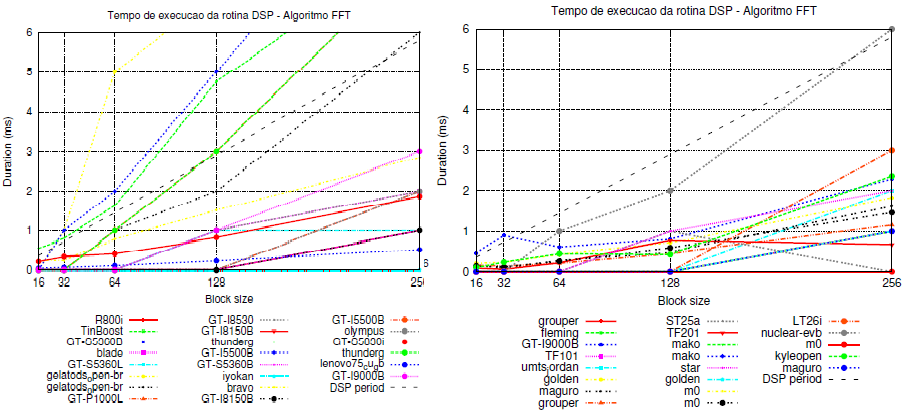
\includegraphics[width=0.5\textwidth]{fft.png}}
  \caption{. Benchmark of FFT Algorithm implemented in pure JAVA}
\end{figure}


\begin{figure}[h!]
  \centering
    \reflectbox{%
      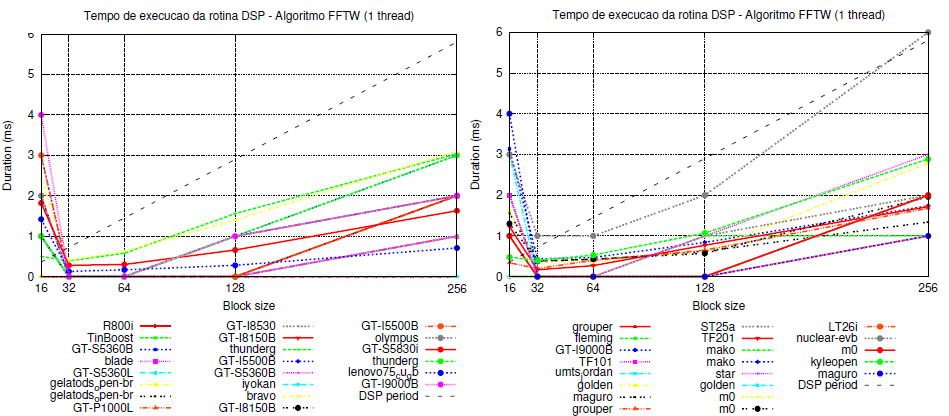
\includegraphics[width=0.5\textwidth]{fftw.png}}
  \caption{. Benchmark of FFTW mono thread}
\end{figure}


\begin{figure}[h!]
  \centering
    \reflectbox{%
      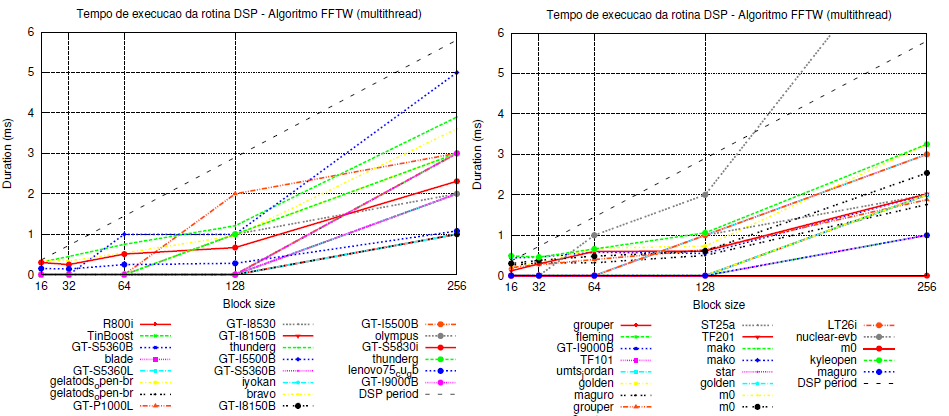
\includegraphics[width=0.5\textwidth]{fftwm.png}}
  \caption{. Benchmark of FFTW multi thread}
\end{figure}


After the benchmark tests we have created some representations to get better
visualization of the performances.  Comparing the FFT benchmark to the FFTW
monothread benchmark, on Figure 1 and Figure 2 respectively, it's possible to
notice that FFTW monothread is faster than FFT when the blocks larger than 16
are considered.  Because of the overhead caused by the loading of a dynamic
library, the results of FFTW monothread for blocks whose size is 16 are worse
than the FFT ones.  As the FFTW library is loaded when the algorithm is
executed for the blocks larger than 16, the overhead due to the initialization
of the library is not noticed for those blocks. The same happens to FFTW
multhread, it is executed after FFTW monothread and therefore there is no
overhead for the initialization of the library.


It's also possible to notice that FFTW ha a worse performance when it is used
with multiple threads. It so happens that kernel of Android shifts the threads
of a program to different cores provided that they are CPU-intensive and has
been running for a sustained period, the threads created by FFTW are
CPU-intensive, however the blocks tested are not large enough to make the
threads be shifted to different cores. In [http://bigflake.com/systrace/]
there some experiments using systrace
[http://developer.android.com/tools/debugging/systrace.html] that point out
what happens to CPU-intensive threads on an Android multicore device. Some
Android devices, like XXX and YYY, have all the cores enabled all the time,
but others, like ZZZ, enable additional cores according to the conditions
explained before. It is said that it happens because turning another core on
is a expensive process in energetic terms, so Android tries to keep 


[ref] 


\subsection{ Conclusion and future work}

\begin{itemize}

    \item FFT perdeu para FFTW


    \item FFTW teve problemas para inicializa��o mas conseguiu superar a FFT
    nos outros casos independente disso
    http://gcc.gnu.org/ml/gcc/2004-06/msg01956.html


    \item Limita��es de dispositivos devem ser consideradas
    http://developer.android.com/training/articles/perf-jni.html\#unsupported


    \item FFTW  multithread n�o superou FFTW mono thread por n�o requisitar
    muito do  processador e assim o processador n�o atribui os processos a
    n�cleos  diferentes 


    \item S� h� vantagem em uso de multithread se o trabalho for muito grande


    \item We  are preparing new tests including FFT to get a better overview
    of other  methods and libraries. Here are the next steps proposed: \# Pure
    Java multithread implementation


    \item FFT from Pure Data using libpd
    (http://puredata.info/downloads/libpd/)  that is a port of Pure Data's
    core engine which make possible to run  Pd patches as C native code over
    Android's Dalvik Java VM. 


    \item FFT from CSound on Android
    \url{http://www.csounds.com/journal/issue17/android\_csd\_player.html}


    \item FFT from supercolider on Android


    \item Testing these methods we will know the state of art on FFT
    implementation for Android devices considering the real time processing
    and also bearing in mind that the fast we compute FFT, the less battery
    draining we will have.

\end{itemize}


\section{Acknowledgements}
We would like to thank the members of the Computer Music Group (http://compmus.ime.usp.br/en/)  of the Computer Science Department of the Institute of Mathematics and  Statistics of the University of S�o Paulo. This work has been supported  by the funding agencies CAPES and FAPESP (grant 2008/08632-8).


\section{References}



\bibliographystyle{apalike}


\bibliography{references}


\end{document}


